\documentclass[tikz,border=9pt]{standalone}
\usepackage{amsmath,amssymb}
\begin{document}
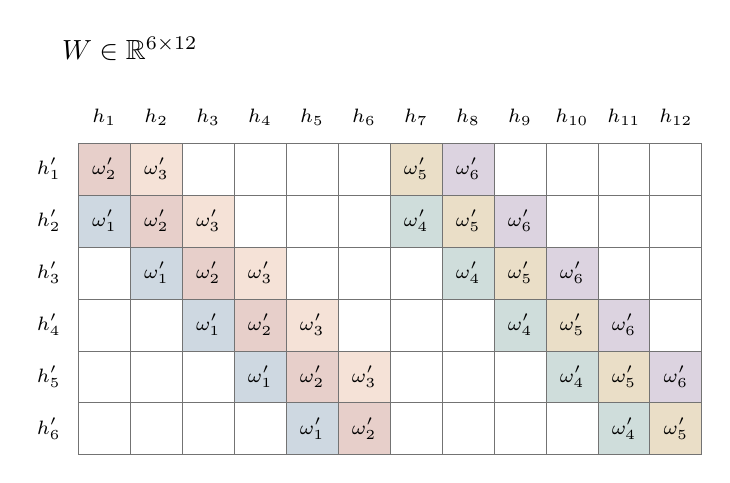
\begin{tikzpicture}
\definecolor{c1}{HTML}{416A8A}
\definecolor{c2}{HTML}{A44732}
\definecolor{c3}{HTML}{D89164}
\definecolor{c4}{HTML}{457C74}
\definecolor{c5}{HTML}{AD7F26}
\definecolor{c6}{HTML}{785789}
\definecolor{c7}{HTML}{BA5F7D}
\definecolor{c8}{HTML}{578AC0}
\definecolor{c9}{HTML}{75943B}
\begin{scope}[shift={(0,0)},x=0.66cm,y=-0.66cm]
\node[anchor=south west] at (-.5,-1.4) {$W\in\mathbb{R}^{6\times12}$};
\node[font=\scriptsize] at (0.5,-.5) {$h_{1}$};
\node[font=\scriptsize] at (1.5,-.5) {$h_{2}$};
\node[font=\scriptsize] at (2.5,-.5) {$h_{3}$};
\node[font=\scriptsize] at (3.5,-.5) {$h_{4}$};
\node[font=\scriptsize] at (4.5,-.5) {$h_{5}$};
\node[font=\scriptsize] at (5.5,-.5) {$h_{6}$};
\node[font=\scriptsize] at (6.5,-.5) {$h_{7}$};
\node[font=\scriptsize] at (7.5,-.5) {$h_{8}$};
\node[font=\scriptsize] at (8.5,-.5) {$h_{9}$};
\node[font=\scriptsize] at (9.5,-.5) {$h_{10}$};
\node[font=\scriptsize] at (10.5,-.5) {$h_{11}$};
\node[font=\scriptsize] at (11.5,-.5) {$h_{12}$};
\node[anchor=east,font=\scriptsize] at (-.15,0.5) {$h^{\prime}_{1}$};
\filldraw[fill=c2!26,draw=black!55,line width=.3pt] (0,0) rectangle ++(1,1);
\node[font=\scriptsize] at (0.5,0.5) {$\omega^{\prime}_{2}$};
\filldraw[fill=c3!26,draw=black!55,line width=.3pt] (1,0) rectangle ++(1,1);
\node[font=\scriptsize] at (1.5,0.5) {$\omega^{\prime}_{3}$};
\filldraw[fill=white,draw=black!55,line width=.3pt] (2,0) rectangle ++(1,1);
\filldraw[fill=white,draw=black!55,line width=.3pt] (3,0) rectangle ++(1,1);
\filldraw[fill=white,draw=black!55,line width=.3pt] (4,0) rectangle ++(1,1);
\filldraw[fill=white,draw=black!55,line width=.3pt] (5,0) rectangle ++(1,1);
\filldraw[fill=c5!26,draw=black!55,line width=.3pt] (6,0) rectangle ++(1,1);
\node[font=\scriptsize] at (6.5,0.5) {$\omega^{\prime}_{5}$};
\filldraw[fill=c6!26,draw=black!55,line width=.3pt] (7,0) rectangle ++(1,1);
\node[font=\scriptsize] at (7.5,0.5) {$\omega^{\prime}_{6}$};
\filldraw[fill=white,draw=black!55,line width=.3pt] (8,0) rectangle ++(1,1);
\filldraw[fill=white,draw=black!55,line width=.3pt] (9,0) rectangle ++(1,1);
\filldraw[fill=white,draw=black!55,line width=.3pt] (10,0) rectangle ++(1,1);
\filldraw[fill=white,draw=black!55,line width=.3pt] (11,0) rectangle ++(1,1);
\node[anchor=east,font=\scriptsize] at (-.15,1.5) {$h^{\prime}_{2}$};
\filldraw[fill=c1!26,draw=black!55,line width=.3pt] (0,1) rectangle ++(1,1);
\node[font=\scriptsize] at (0.5,1.5) {$\omega^{\prime}_{1}$};
\filldraw[fill=c2!26,draw=black!55,line width=.3pt] (1,1) rectangle ++(1,1);
\node[font=\scriptsize] at (1.5,1.5) {$\omega^{\prime}_{2}$};
\filldraw[fill=c3!26,draw=black!55,line width=.3pt] (2,1) rectangle ++(1,1);
\node[font=\scriptsize] at (2.5,1.5) {$\omega^{\prime}_{3}$};
\filldraw[fill=white,draw=black!55,line width=.3pt] (3,1) rectangle ++(1,1);
\filldraw[fill=white,draw=black!55,line width=.3pt] (4,1) rectangle ++(1,1);
\filldraw[fill=white,draw=black!55,line width=.3pt] (5,1) rectangle ++(1,1);
\filldraw[fill=c4!26,draw=black!55,line width=.3pt] (6,1) rectangle ++(1,1);
\node[font=\scriptsize] at (6.5,1.5) {$\omega^{\prime}_{4}$};
\filldraw[fill=c5!26,draw=black!55,line width=.3pt] (7,1) rectangle ++(1,1);
\node[font=\scriptsize] at (7.5,1.5) {$\omega^{\prime}_{5}$};
\filldraw[fill=c6!26,draw=black!55,line width=.3pt] (8,1) rectangle ++(1,1);
\node[font=\scriptsize] at (8.5,1.5) {$\omega^{\prime}_{6}$};
\filldraw[fill=white,draw=black!55,line width=.3pt] (9,1) rectangle ++(1,1);
\filldraw[fill=white,draw=black!55,line width=.3pt] (10,1) rectangle ++(1,1);
\filldraw[fill=white,draw=black!55,line width=.3pt] (11,1) rectangle ++(1,1);
\node[anchor=east,font=\scriptsize] at (-.15,2.5) {$h^{\prime}_{3}$};
\filldraw[fill=white,draw=black!55,line width=.3pt] (0,2) rectangle ++(1,1);
\filldraw[fill=c1!26,draw=black!55,line width=.3pt] (1,2) rectangle ++(1,1);
\node[font=\scriptsize] at (1.5,2.5) {$\omega^{\prime}_{1}$};
\filldraw[fill=c2!26,draw=black!55,line width=.3pt] (2,2) rectangle ++(1,1);
\node[font=\scriptsize] at (2.5,2.5) {$\omega^{\prime}_{2}$};
\filldraw[fill=c3!26,draw=black!55,line width=.3pt] (3,2) rectangle ++(1,1);
\node[font=\scriptsize] at (3.5,2.5) {$\omega^{\prime}_{3}$};
\filldraw[fill=white,draw=black!55,line width=.3pt] (4,2) rectangle ++(1,1);
\filldraw[fill=white,draw=black!55,line width=.3pt] (5,2) rectangle ++(1,1);
\filldraw[fill=white,draw=black!55,line width=.3pt] (6,2) rectangle ++(1,1);
\filldraw[fill=c4!26,draw=black!55,line width=.3pt] (7,2) rectangle ++(1,1);
\node[font=\scriptsize] at (7.5,2.5) {$\omega^{\prime}_{4}$};
\filldraw[fill=c5!26,draw=black!55,line width=.3pt] (8,2) rectangle ++(1,1);
\node[font=\scriptsize] at (8.5,2.5) {$\omega^{\prime}_{5}$};
\filldraw[fill=c6!26,draw=black!55,line width=.3pt] (9,2) rectangle ++(1,1);
\node[font=\scriptsize] at (9.5,2.5) {$\omega^{\prime}_{6}$};
\filldraw[fill=white,draw=black!55,line width=.3pt] (10,2) rectangle ++(1,1);
\filldraw[fill=white,draw=black!55,line width=.3pt] (11,2) rectangle ++(1,1);
\node[anchor=east,font=\scriptsize] at (-.15,3.5) {$h^{\prime}_{4}$};
\filldraw[fill=white,draw=black!55,line width=.3pt] (0,3) rectangle ++(1,1);
\filldraw[fill=white,draw=black!55,line width=.3pt] (1,3) rectangle ++(1,1);
\filldraw[fill=c1!26,draw=black!55,line width=.3pt] (2,3) rectangle ++(1,1);
\node[font=\scriptsize] at (2.5,3.5) {$\omega^{\prime}_{1}$};
\filldraw[fill=c2!26,draw=black!55,line width=.3pt] (3,3) rectangle ++(1,1);
\node[font=\scriptsize] at (3.5,3.5) {$\omega^{\prime}_{2}$};
\filldraw[fill=c3!26,draw=black!55,line width=.3pt] (4,3) rectangle ++(1,1);
\node[font=\scriptsize] at (4.5,3.5) {$\omega^{\prime}_{3}$};
\filldraw[fill=white,draw=black!55,line width=.3pt] (5,3) rectangle ++(1,1);
\filldraw[fill=white,draw=black!55,line width=.3pt] (6,3) rectangle ++(1,1);
\filldraw[fill=white,draw=black!55,line width=.3pt] (7,3) rectangle ++(1,1);
\filldraw[fill=c4!26,draw=black!55,line width=.3pt] (8,3) rectangle ++(1,1);
\node[font=\scriptsize] at (8.5,3.5) {$\omega^{\prime}_{4}$};
\filldraw[fill=c5!26,draw=black!55,line width=.3pt] (9,3) rectangle ++(1,1);
\node[font=\scriptsize] at (9.5,3.5) {$\omega^{\prime}_{5}$};
\filldraw[fill=c6!26,draw=black!55,line width=.3pt] (10,3) rectangle ++(1,1);
\node[font=\scriptsize] at (10.5,3.5) {$\omega^{\prime}_{6}$};
\filldraw[fill=white,draw=black!55,line width=.3pt] (11,3) rectangle ++(1,1);
\node[anchor=east,font=\scriptsize] at (-.15,4.5) {$h^{\prime}_{5}$};
\filldraw[fill=white,draw=black!55,line width=.3pt] (0,4) rectangle ++(1,1);
\filldraw[fill=white,draw=black!55,line width=.3pt] (1,4) rectangle ++(1,1);
\filldraw[fill=white,draw=black!55,line width=.3pt] (2,4) rectangle ++(1,1);
\filldraw[fill=c1!26,draw=black!55,line width=.3pt] (3,4) rectangle ++(1,1);
\node[font=\scriptsize] at (3.5,4.5) {$\omega^{\prime}_{1}$};
\filldraw[fill=c2!26,draw=black!55,line width=.3pt] (4,4) rectangle ++(1,1);
\node[font=\scriptsize] at (4.5,4.5) {$\omega^{\prime}_{2}$};
\filldraw[fill=c3!26,draw=black!55,line width=.3pt] (5,4) rectangle ++(1,1);
\node[font=\scriptsize] at (5.5,4.5) {$\omega^{\prime}_{3}$};
\filldraw[fill=white,draw=black!55,line width=.3pt] (6,4) rectangle ++(1,1);
\filldraw[fill=white,draw=black!55,line width=.3pt] (7,4) rectangle ++(1,1);
\filldraw[fill=white,draw=black!55,line width=.3pt] (8,4) rectangle ++(1,1);
\filldraw[fill=c4!26,draw=black!55,line width=.3pt] (9,4) rectangle ++(1,1);
\node[font=\scriptsize] at (9.5,4.5) {$\omega^{\prime}_{4}$};
\filldraw[fill=c5!26,draw=black!55,line width=.3pt] (10,4) rectangle ++(1,1);
\node[font=\scriptsize] at (10.5,4.5) {$\omega^{\prime}_{5}$};
\filldraw[fill=c6!26,draw=black!55,line width=.3pt] (11,4) rectangle ++(1,1);
\node[font=\scriptsize] at (11.5,4.5) {$\omega^{\prime}_{6}$};
\node[anchor=east,font=\scriptsize] at (-.15,5.5) {$h^{\prime}_{6}$};
\filldraw[fill=white,draw=black!55,line width=.3pt] (0,5) rectangle ++(1,1);
\filldraw[fill=white,draw=black!55,line width=.3pt] (1,5) rectangle ++(1,1);
\filldraw[fill=white,draw=black!55,line width=.3pt] (2,5) rectangle ++(1,1);
\filldraw[fill=white,draw=black!55,line width=.3pt] (3,5) rectangle ++(1,1);
\filldraw[fill=c1!26,draw=black!55,line width=.3pt] (4,5) rectangle ++(1,1);
\node[font=\scriptsize] at (4.5,5.5) {$\omega^{\prime}_{1}$};
\filldraw[fill=c2!26,draw=black!55,line width=.3pt] (5,5) rectangle ++(1,1);
\node[font=\scriptsize] at (5.5,5.5) {$\omega^{\prime}_{2}$};
\filldraw[fill=white,draw=black!55,line width=.3pt] (6,5) rectangle ++(1,1);
\filldraw[fill=white,draw=black!55,line width=.3pt] (7,5) rectangle ++(1,1);
\filldraw[fill=white,draw=black!55,line width=.3pt] (8,5) rectangle ++(1,1);
\filldraw[fill=white,draw=black!55,line width=.3pt] (9,5) rectangle ++(1,1);
\filldraw[fill=c4!26,draw=black!55,line width=.3pt] (10,5) rectangle ++(1,1);
\node[font=\scriptsize] at (10.5,5.5) {$\omega^{\prime}_{4}$};
\filldraw[fill=c5!26,draw=black!55,line width=.3pt] (11,5) rectangle ++(1,1);
\node[font=\scriptsize] at (11.5,5.5) {$\omega^{\prime}_{5}$};
\end{scope}

\end{tikzpicture}
\end{document}
